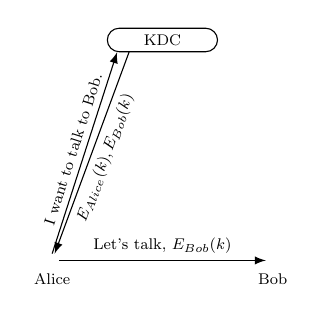
\begin{tikzpicture}[font=\footnotesize,scale=0.7, every node/.style={scale=0.7}]
\node (A) at (0,0) [label=below:Alice] {\Alice};
\node (B) [right of = A, node distance = 4cm,label=below:Bob] {\Bob};
\node (KDC) at (2,4) [rounded corners=1ex,minimum width=2cm,draw] {KDC};  
\draw[-latex] (A) -- (B) node [midway,above] {Let's talk, $E_{Bob}(k)$};
\draw[-latex] (A.90) -- (KDC.195) node [sloped,midway,above] {I want to talk to Bob.};
\draw[-latex] (KDC.200) -- (A.70) node [sloped,midway,below] {$E_{Alice}(k),E_{Bob}(k)$};
\end{tikzpicture}